\section{Insiemi}
Gli insiemi sono definibili come delle correlazioni di elementi e saranno alla base del corso di FDI. \footnote{Ricorda che all'interno di un insieme gli elementi possono essere ripetuti, in tal caso per le varie operazioni da fare questi elementi ripetuti andranno considerati come unici} \\ \\
\textbf{Cardinalità}: si rappresenta con n o \(|A|\) ed è uno dei paramenti di un insieme ed è il numero di elementi nell'insieme. \\ \\
Gli insiemi possono inoltre essere finiti o infiniti.\\
\textbf{Finiti}: quando hanno un numero finito di elementi.\\
\textbf{Infiniti}: quando invece il numero di elementi è infinito.
\begin{example}
Esempi insiemi finiti ed infiniti:
\begin{itemize}
    \item Insieme finito: \(A = \{a_1, a_2, a_3, ..., a_n \}\) \(|A| = n\). \footnote{I tre puntini '...' si utilizzano quando non si è in grado di scrivere tutti gli elementi}
    \item Insieme finito: \(GS = \{lun, mar, mer, ..., dom\}\) \(|GS| = 7\).
    \item Insieme infinito: \(A = \{..., a_i-1, a_i, a_i+1, ...\}\) \(|A| = \infty\).
\end{itemize}
\end{example}

\subsection{Notazione}
\textbf{Elementi:} Lettere piccole dell'alfabeto. Ess: a, b, c - \(a_1, a_2, a_3\) \\
\textbf{Insiemi:} Lettere maiuscole dell'alfabeto. Ess: A, B, C \\
\textbf{Appartiene:} \(a \in A\) \hspace { 1cm } \textbf{Non Appartiene:} \(a \notin A\) \hspace { 1cm } \textbf{Tale che:} $|$ 
\begin{example}
Alcuni insiemi infiniti ricorrenti:\\
\(\mathbb{N}\) = num. naturali \hspace{.5cm} \(\mathbb{Z}\) = num. interi \hspace{.5cm} \(\mathbb{Q}\) = num. razionali \hspace{.5cm} \(\mathbb{R}\) = num. reali
\end{example}

\subsection{Specificare un insieme}
Un insieme può essere scritto sotto due forme, quella estensionale e quella intenzionale.
\begin{itemize}
    \item \textbf{Estensionale} o per enumerazione: si va ad elencare esplicitamente tutti gli oggetti.
    \begin{example}
        Esempi estensionale:\\
        \(ore = \{1, 2, 3, ..., 24\}\)  -  \(vocali = \{a, e, i, o, u\}\) \\
        $n = \{0, 1, 2, ..., n-1\}$  -  $\O = \{\}$ (insieme vuoto)
    \end{example}
    \item \textbf{Intenzionale} o per proprietà: si va ad elencare implicitamente tutti gli oggetti attraverso una regola che li caratterizza.
    \begin{example}
        Esempi intenzionale:\\
        $ore_1 = \{n \in \mathbb{N} \:|\: n \geq\ 1$ and $n \leq 24\}$ \hspace{.7cm} $N_p = \{n \in \mathbb{N} \:|\: n$ è divisibile per 2 $\}$ \\
        $N_d = \{n \in \mathbb{N} \:|\: n$ non è divisibile per 2$\}$ \hspace{.7cm} $\mathbb{Q} = \{n/m \:|\: n \in \mathbb{Z}, \, m \in \mathbb{N}$, ma $ m \neq 0\}$
    \end{example}
\end{itemize}

\newpage
\subsection{Proprietà degli insiemi}
\subsubsection{Confrontare due insiemi}
$A = B$ se contengono esattamente gli stessi elementi.\\
$A \neq B$ almeno un elemento di A non occorre in B oppure almeno un elemento di B non occorre in A.\\\\
\textbf{Domanda:} Con $A = \{a, e, b, c, o, u\}$ e $B = \{a, b, e, b, c, o, o, u\}$, $A = B$ ?\\
Se partiamo dalla definizione di insiemi uguali, cioè che A = B quando A contiene gli stessi elementi di B e viceversa possiamo concludere che SI in questa casistica A e B sono uguali. \\
Da qui possiamo definire una \textbf{proprietà del confronto}:
A = B equivale a dire che ogni elemento di $a \in A$ e anche $a \in B$ e ogni elemento $b \in B$ è anche $b \in A$. \\
Inoltre, continuando su questo ragionamento possiamo anche vedere come la cardinalità di due insiemi uguali non necessariamente è uguale.

\subsubsection{Inclusione fra insiemi}
\begin{wrapfigure}{r}{5.5cm}
    \vspace{-10pt}
    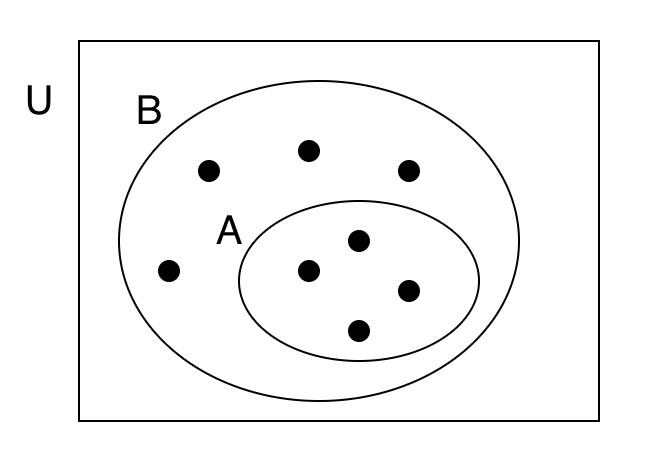
\includegraphics[width=6cm]{Eulero-venn-contenuto-uguale.png}
    \caption{Contenuto uguale}
    \label{fig:contenuto-uguale}
\end{wrapfigure}
\textbf{Contenuto uguale:} $A \subseteq B$ \hspace{.3cm} Figura [\ref{fig:contenuto-uguale}] \\(Ogni elemento di A è anche elemento di B e possono essere uguali, ma non necessariamente) \\
$A \subseteq U$ \hspace{.3cm} $A \subseteq B$ \hspace{.3cm} $B \subseteq U$ \footnote{con il simbolo "U", chiamato universo, si indicano tutti i possibili elementi che possiamo trovare in un insieme.} \\ \\
\textbf{Inclusione impropria e stretta:} $A \subset B$ \hspace{.2cm} \\(da usare solo quando vuoi specificare che $A \neq B$) \\
Proprietà: Per ogni insieme di A si ha che:\\
$\O \subseteq A$ \hspace{.2cm} $A \subseteq U$ \\ \\
\textbf{Insiemi disgiunti:} A e B si dicono insiemi disgiunti quando non hanno elementi in comune: \\
$\{$non esiste $x \in U \: | \: x \in A \: and \: x \in B\}$\\

\subsubsection{Proprietà di uguaglianza ed inclusione}
Per tutti gli insiemi A, B, C valgono le proprietà scritte in tabella \ref{tab:proprietà-uguaglianza-inclusione}.
\begin{table}[h!]
    \vspace{10pt}
    \centering
    \setlength{\tabcolsep}{7pt}
    \renewcommand{\arraystretch}{2.5}
    \begin{tabular}{|c|c|c|}
        \hline
        \textbf{Riflessiva} & A = A & $A \subseteq A$ \\ \hline
        \textbf{Transitiva} & Se A = B e B = C allora A = C & Se $A \subseteq B$ e $B \subseteq C$ allora  $A \subseteq C$\\ \hline
        \textbf{Simmetrica} & Se A = B allora B = A & \textit{Niente} \\ \hline
        \textbf{Antisimmetrica} & \textit{Niente} & Se $A \subseteq B$ e $B \subseteq A$ allora A = B \\
        \hline
    \end{tabular}
    \caption{Proprietà Uguaglianza ed Inclusione}
    \label{tab:proprietà-uguaglianza-inclusione}
\end{table}

\newpage
\subsection{Operazioni su insiemi}
\textbf{Cardinalità:} (solo per insiemi finiti) si indica con $|A|$
\begin{example}
    Esempi cardinalità:\\
    $|\overline{A}| = |U| - |A|$ \hspace{.6cm} $|A \cup B| = |A| + |B| - |A \cap B|$ \hspace{.6cm} $|A \setminus B| = |A| - |A \cap B|$\\
\end{example}
\hspace{-15pt}\textbf{Unione:} $A \cup B = \{x \in U \: | \: x \in A \: or \: x \in B\}$ \hfill
\textbf{Intersezione:} $A \cup B = \{x \in U \: | \: x \in A \: or \: x \in B\}$
\begin{figure}[h!]
    \vspace{-7pt}
    \begin{subfigure}{.5\textwidth}
        \centering
        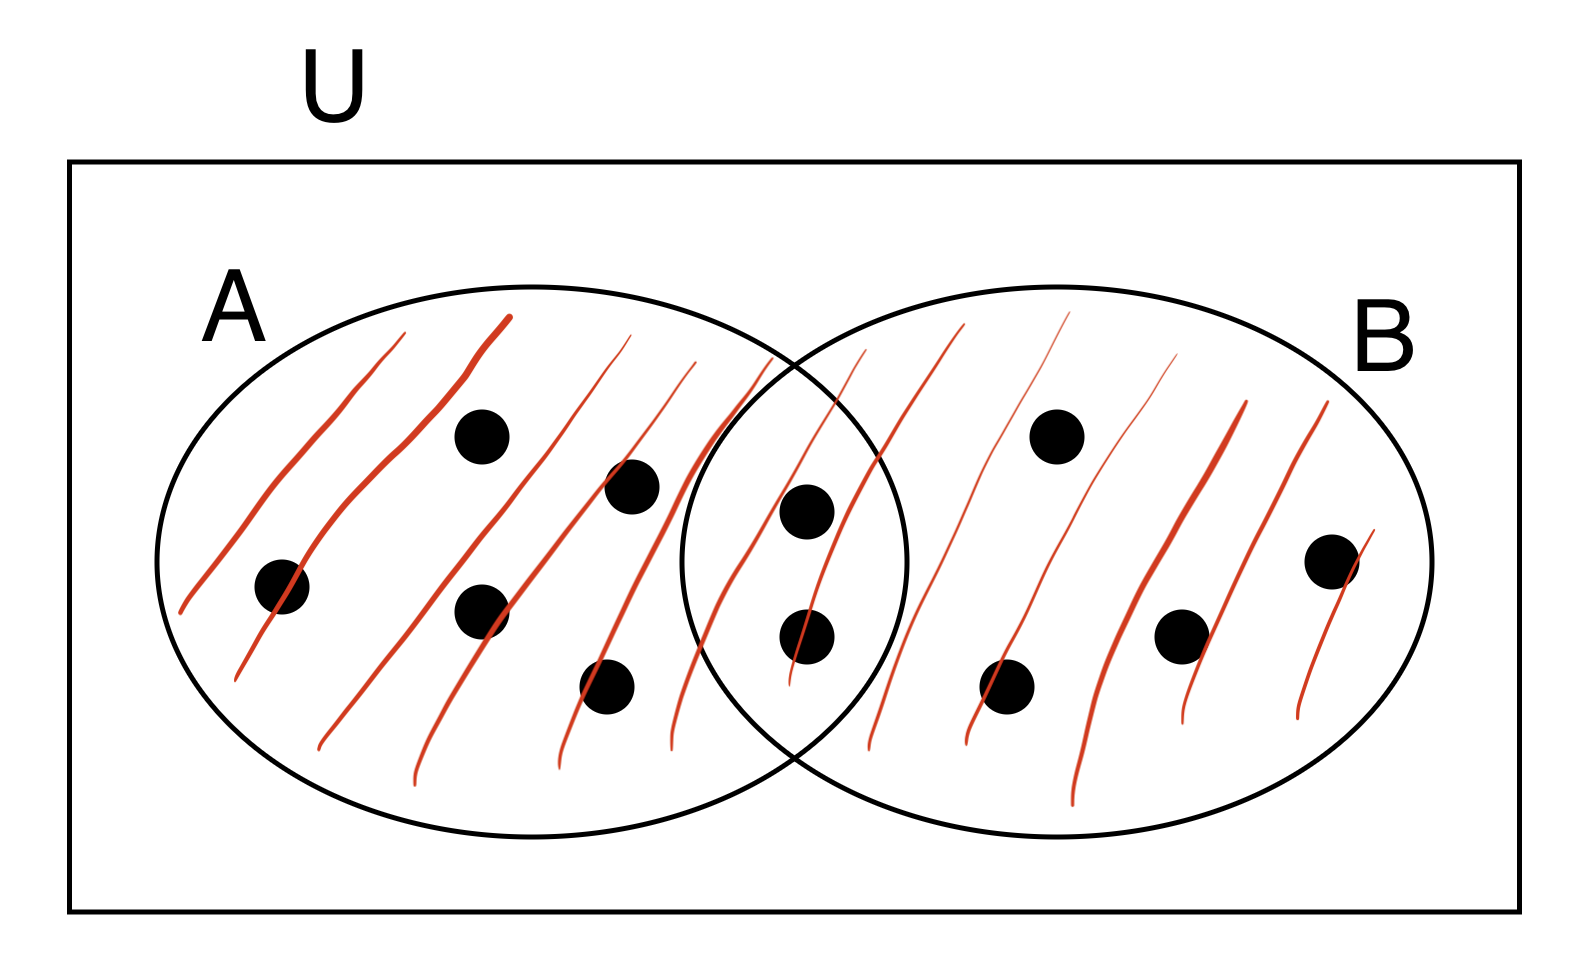
\includegraphics[width=5cm]{Unione.png}
        \caption{Unione}
        \label{fig:unione}
    \end{subfigure}
    \begin{subfigure}{.5\textwidth}
        \centering
        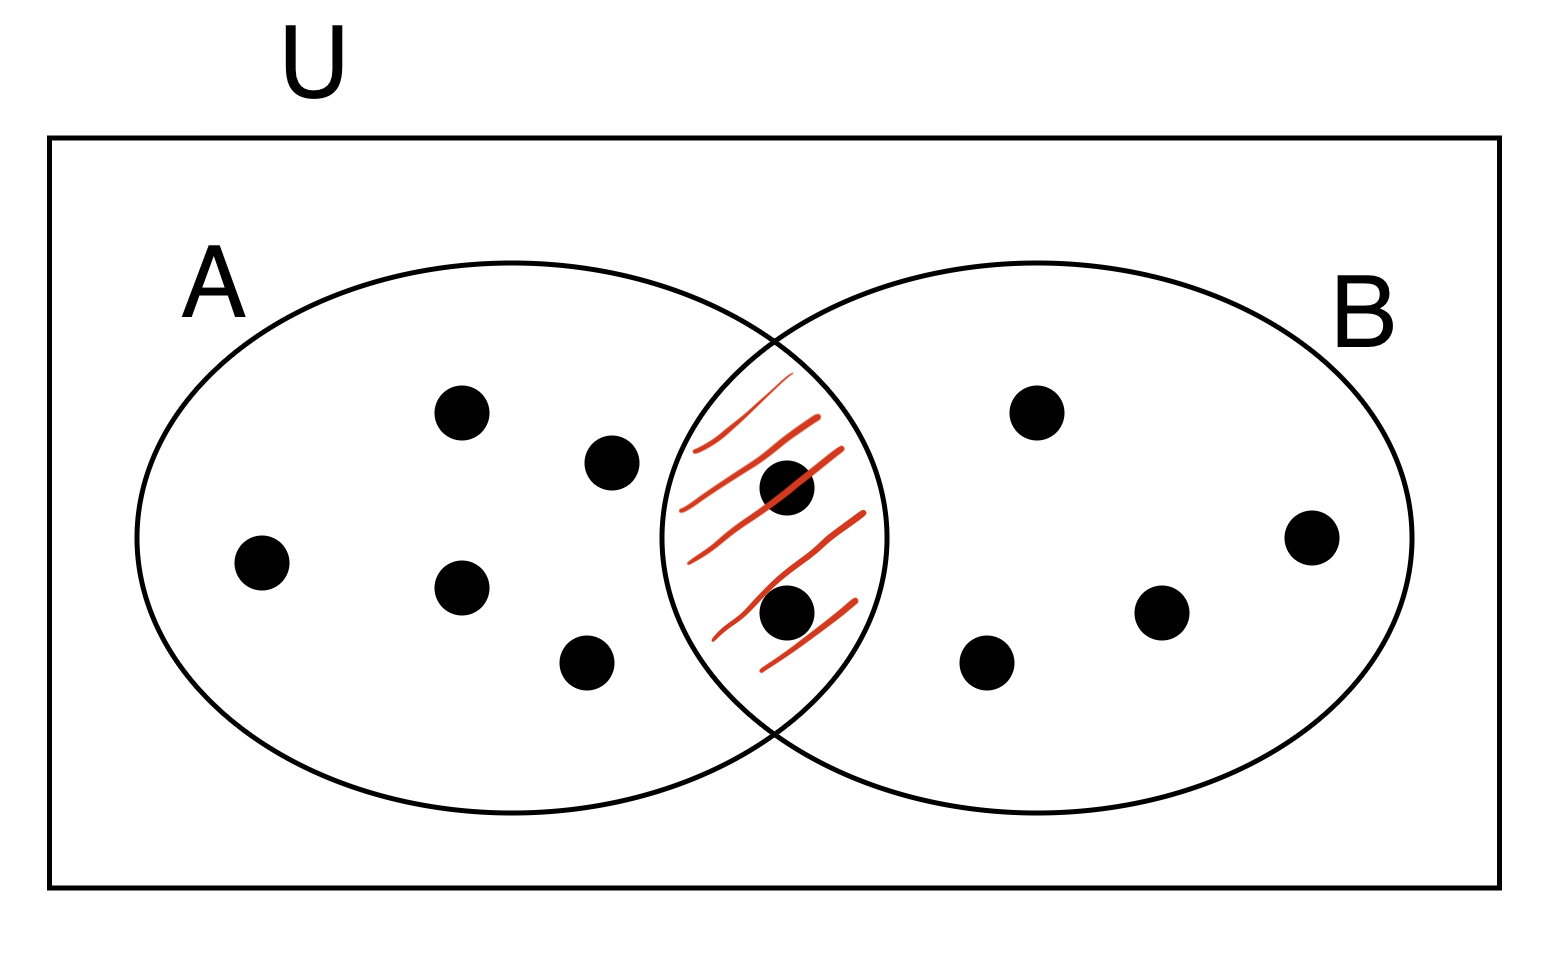
\includegraphics[width=5cm]{Intersezione.png}
        \caption{Intersezione}
        \label{fig:intesezione}
    \end{subfigure}
\end{figure}
\\
\textbf{Differenza:} $A \setminus B = \{x \in U \: | \: x \in A \: and \: x \notin B\}$\hspace{1cm}
\textbf{Complemento:} $\overline{A} = \{c \in U \: | \: x \notin A\}$
\begin{figure}[h!]
        \vspace{-10pt}
    \begin{subfigure}{.5\textwidth}
        \centering
        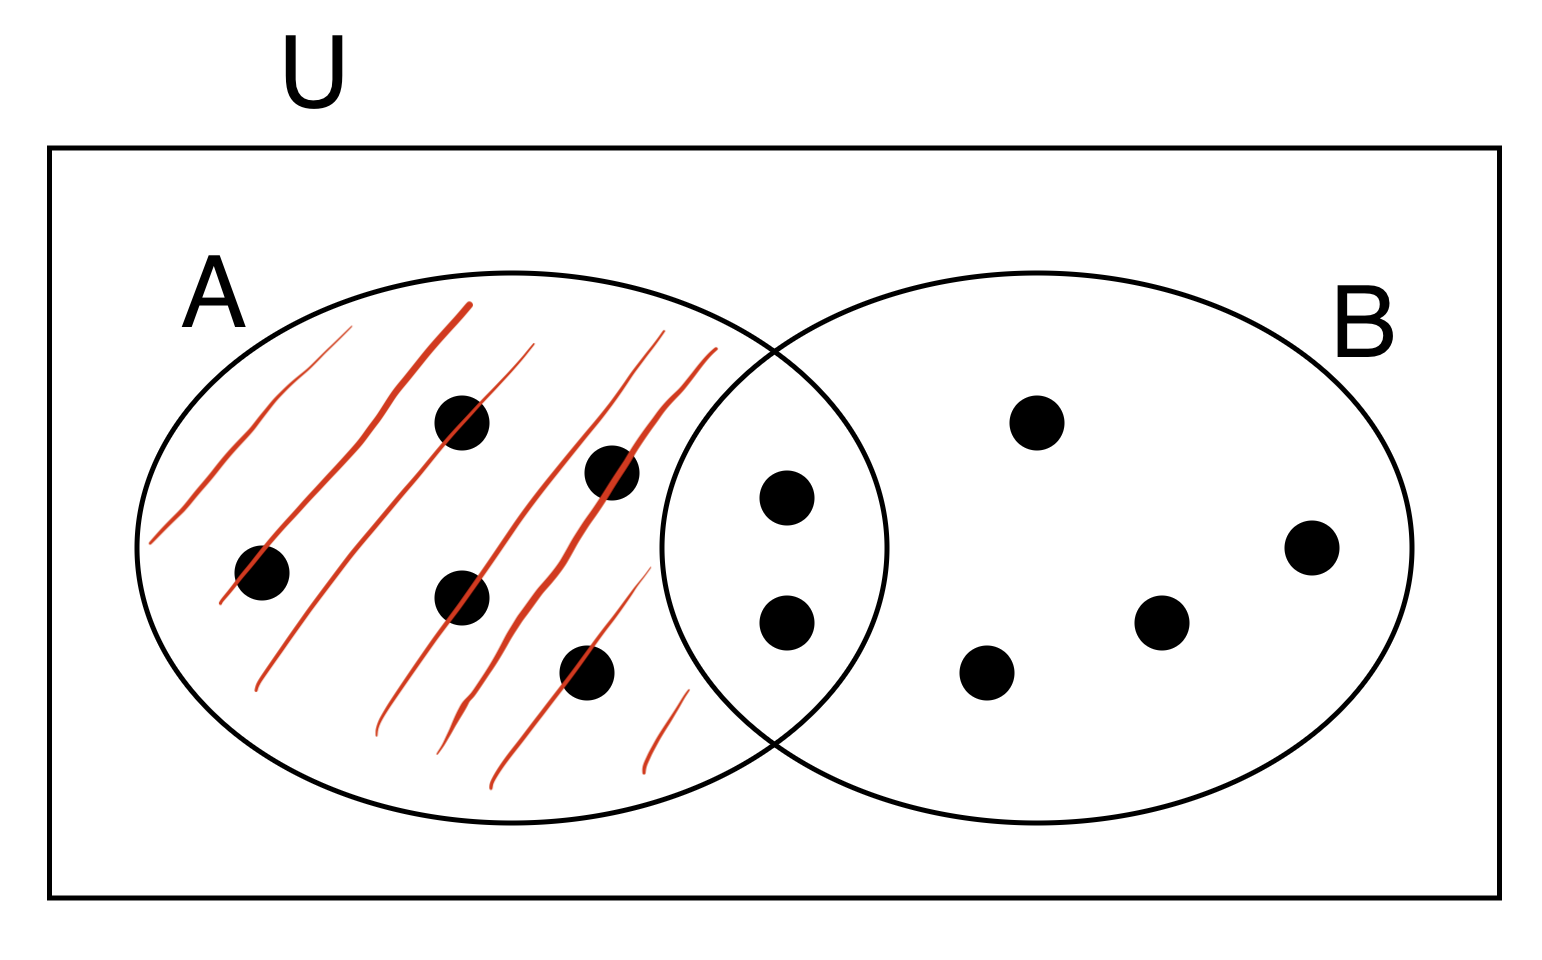
\includegraphics[width=5cm]{Differenza.png}
        \caption{Differenza}
        \label{fig:differenza}
    \end{subfigure}
    \begin{subfigure}{.5\textwidth}
        \centering
        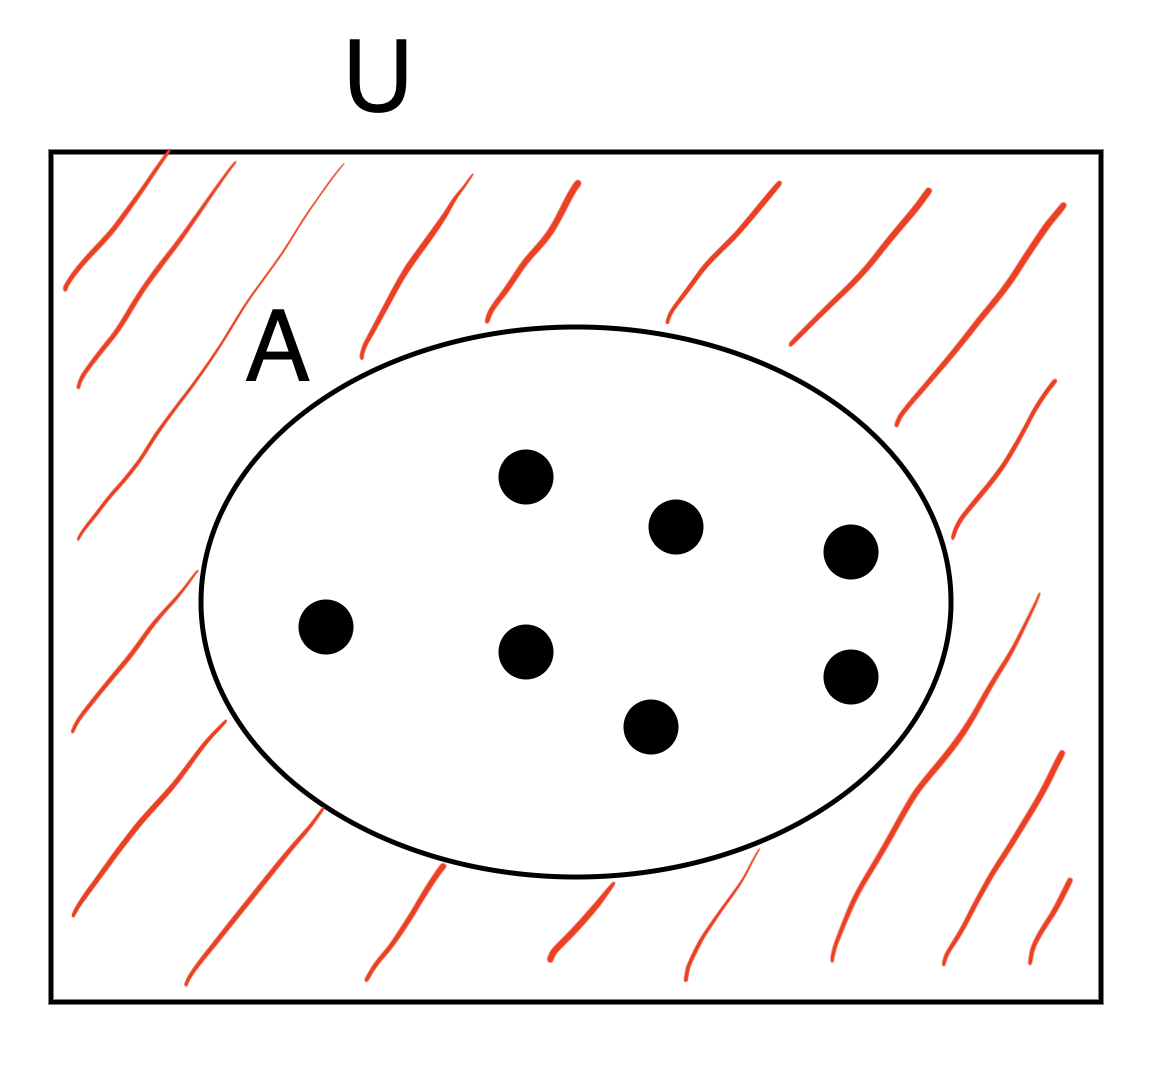
\includegraphics[width=4cm]{Complemento.png}
        \caption{Complemento}
        \label{fig:complemento}
    \end{subfigure}
\end{figure}

\vspace{-5pt}
\subsection{Tavola delle leggi}
Per tutti gli insieme A, B, C (dell'universo \textit{U}) valgono le uguaglianze nella tabella \ref{tab:leggi-insiemi}
\begin{table}[h!]
    \centering
    \setlength{\tabcolsep}{8pt}
    \renewcommand{\arraystretch}{2}
    \begin{tabular}{|c|c c|}
        \hline
        \textbf{Associazione} & $A \cup (B \cup C) = (A \cup B) \cup C$ & $A \cap (B \cap C) = (A \cap B) \cap C$ \\
        \textbf{Unita} & $A \cup \O = A$ & $A \cap U = A$ \\
        \textbf{Commutativa} & $A \cup B = B \cup A$ & $A \cap B = B \cap A$ \\
        \textbf{Indipendenza} & $A \cup A = A$ & $A \cap A = A$ \\
        \textbf{Assorbimento} & $A \cup U = U$ & $A \cap \O = \O$ \\
        \textbf{Distributiva} & $A \cup (B \cap C) = (A \cup B) \cap (A \cup C)$ & $A \cap (B \cup C) = (A \cap B) \cup (A \cap C)$ \\
        \textbf{Complemento} & $A \cup \overline{A} = U$ & $A \cap \overline{A} = \O$ \\
        \textbf{De Morgan} & $\overline{A \cup B} = \overline{A} \cap \overline{B}$ & $\overline{A \cap B} = \overline{A} \cup \overline{B}$ \\
        \textbf{Convoluzione} & $\overline{(\overline{A})} = A$ &  \\
        \textbf{Assrbimento con $\cap$ e $\cup$} & $A \cup (A \cap B) = A$ & $A \cap (A \cup B) = A$ \\
        \hline
    \end{tabular}
    \caption{Tavola delle leggi}
    \label{tab:leggi-insiemi}
\end{table}

\newpage
\subsection{Algebra di Bool}
L'algebra di bool sta alla base dell'informatica e si compone di solo 2 elementi che possono essere rappresentati in tanti modi: V - F, Vero - Falso, True - False, 1 - 0, $\O$ - U \\ \\
Su questi elementi possono essere applicate una serie di operazioni che sono: \\
\textbf{And}, \&\&, $\land$ \hspace{.3cm} \textbf{Or}, $||$, $\lor$ \hspace{.3cm} \textbf{Not}, $\sim$, $\lnot$
\textbf{Implicazione:}\footnote{La parte a sinistra della freccia si chiama \textbf{premessa}, la parte a destra invece \textbf{conseguenza}} $A \Longrightarrow B$, se $A$ allora $B$ \\
\textbf{Conseguenza:} $A \Longleftarrow B$, $A$ se $B$ \\ 
\textbf{Doppia implicazione:} $A \iff B$, $A$ se e solo se $B$

\begin{table}[h!]
    \centering
    \setlength{\tabcolsep}{10pt}
    \renewcommand{\arraystretch}{1.5}
    \begin{tabular}{c|c|c|c|c|c|c|c}
        A & B & $A \land B$ & $A \lor B$ & $\lnot A$ & $A \Longrightarrow B$ & $A \Longleftarrow B$ & $A \iff B$\\
        \hline
        \O & \O & \O & \O & U & U & U & U\\
        \O & U & \O & U & U & U & \O & \O\\ 
        U & \O & \O & U & \O & \O & U & \O\\ 
        U & U & U & U & \O & U & U & U
    \end{tabular}
    \caption{Operazioni con algebra booleana}
\end{table}
\begin{note}
Se nella tabella andiamo a sostituire lo \O \: con 0 e U con 1 o con qualsiasi altro valore corrispondente nell'algebra di boole il risultato resta invariato.
\end{note}

\subsection{Dimostrazioni}
Una \textbf{legge} è \textbf{valida} se vale per tutte le scelte dell'insieme che prendiamo in considerazione. Una \textbf{dimostrazione} indica la validità di una legge. Un \textbf{controesempio} mostra che la legge non è valida per ogni possibilità.
Ci sono 3 tecniche di dimostrazione: \textbf{grafica} (diagramma di Eulero-Venn), \textbf{discorsiva} e tramite \textbf{sostituzione}

\subsubsection{Grafica}
\begin{example}
    Dimostriamo la legge distributiva mediamente i diagrammi di Eulero-Venn.
    \begin{equation}
    	A \cup (B \cap C) = (A \cup B) \cap (A \cup C)
    \end{equation}
	%TODO inserire il titolo per la serie di diagrammi: prima il lato sinistro della dimostrazione e poi il lato destro
    \begin{figure}[h!]
        \begin{subfigure}{.3\textwidth}
            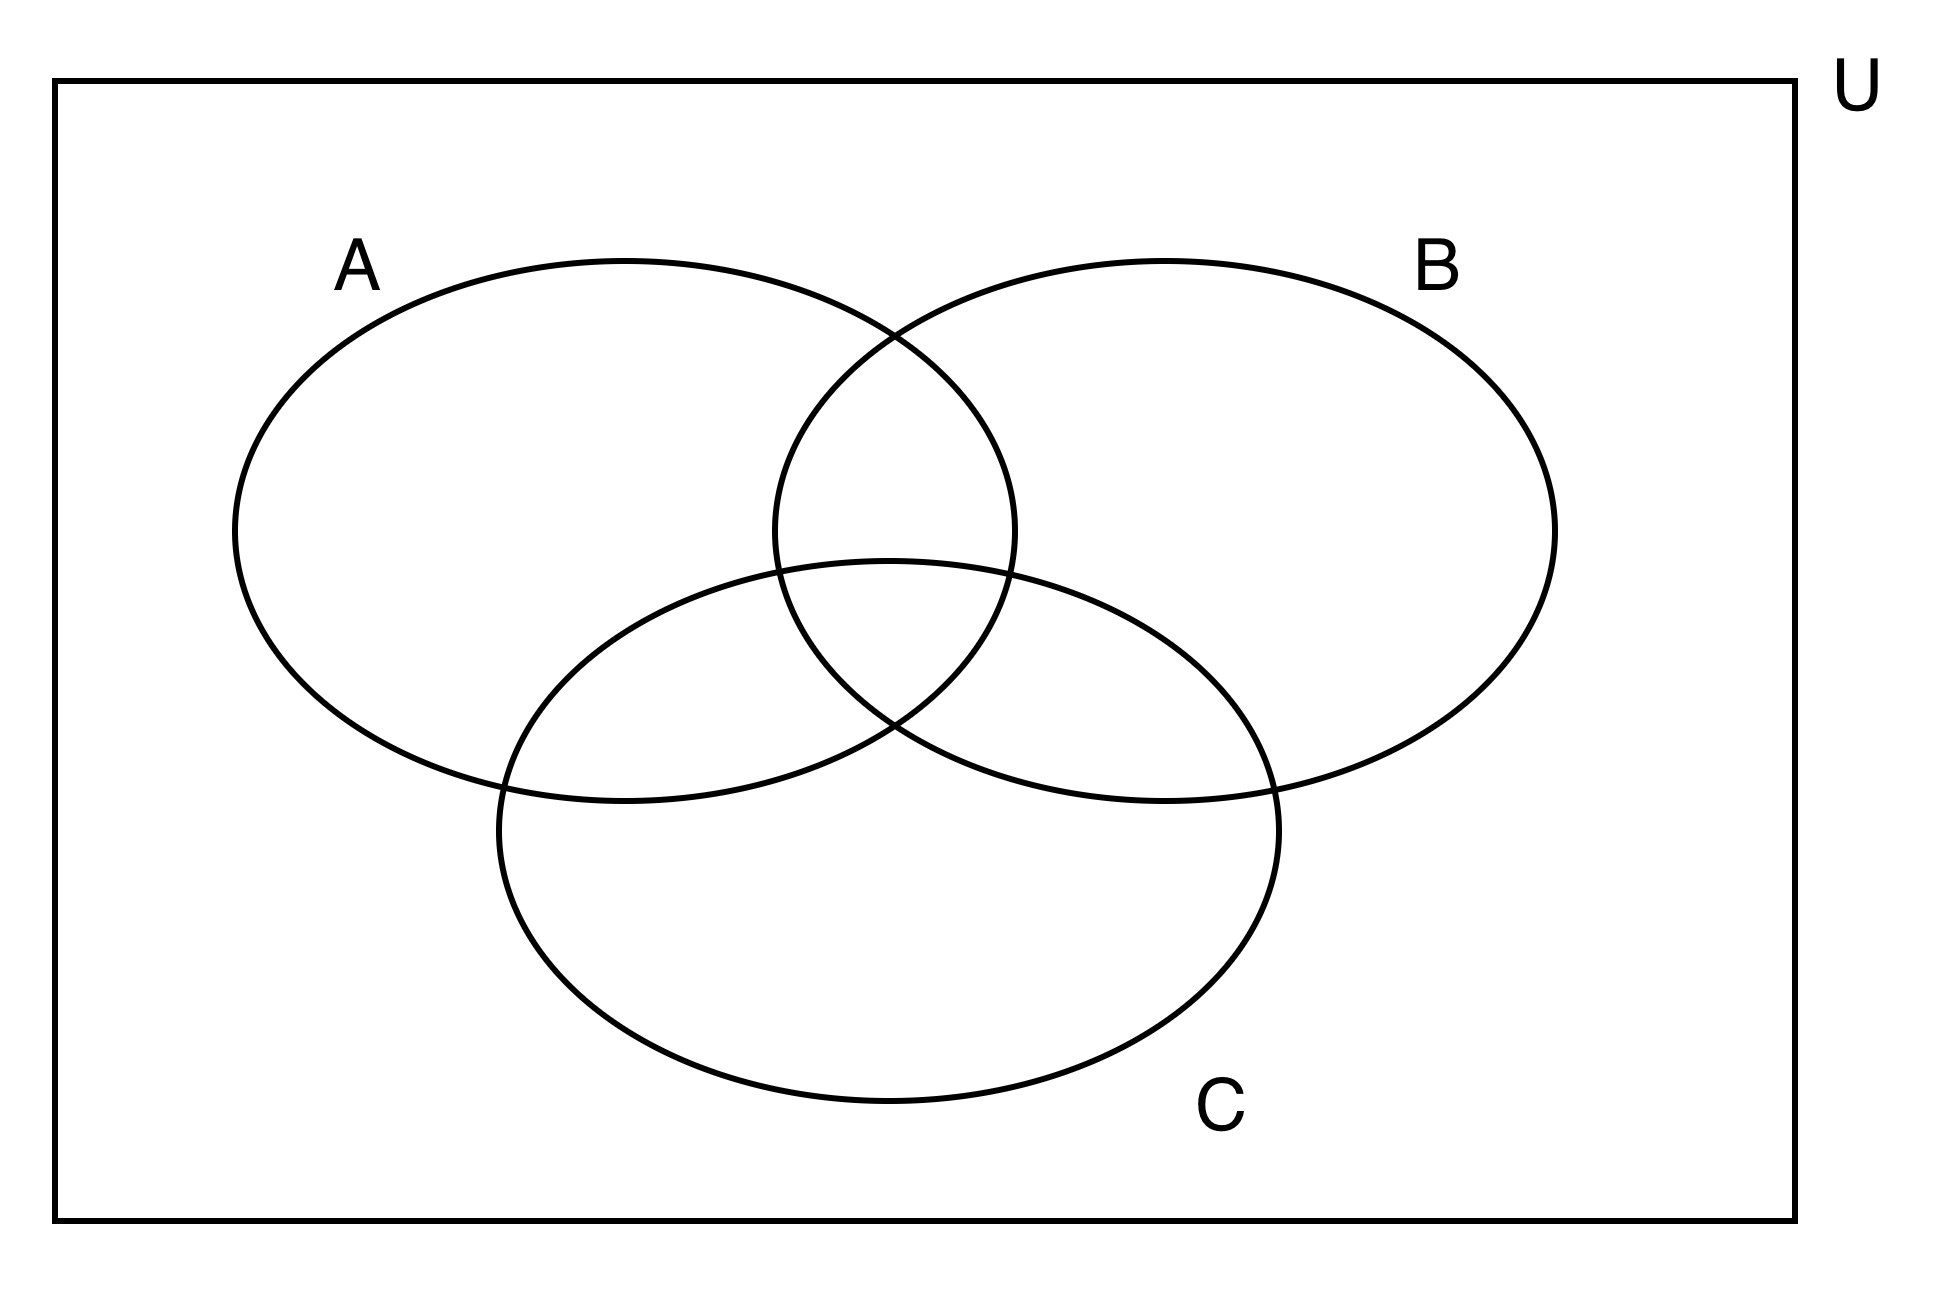
\includegraphics[width=4cm]{Dimostrazione-distibutiva-eulero-venn-1.png}
            \caption{Insiemi di partenza}
            \label{fig:Dimostrazione-distibutiva-eulero-venn-1}
        \end{subfigure}
        \hfill
        \begin{subfigure}{.3\textwidth}
            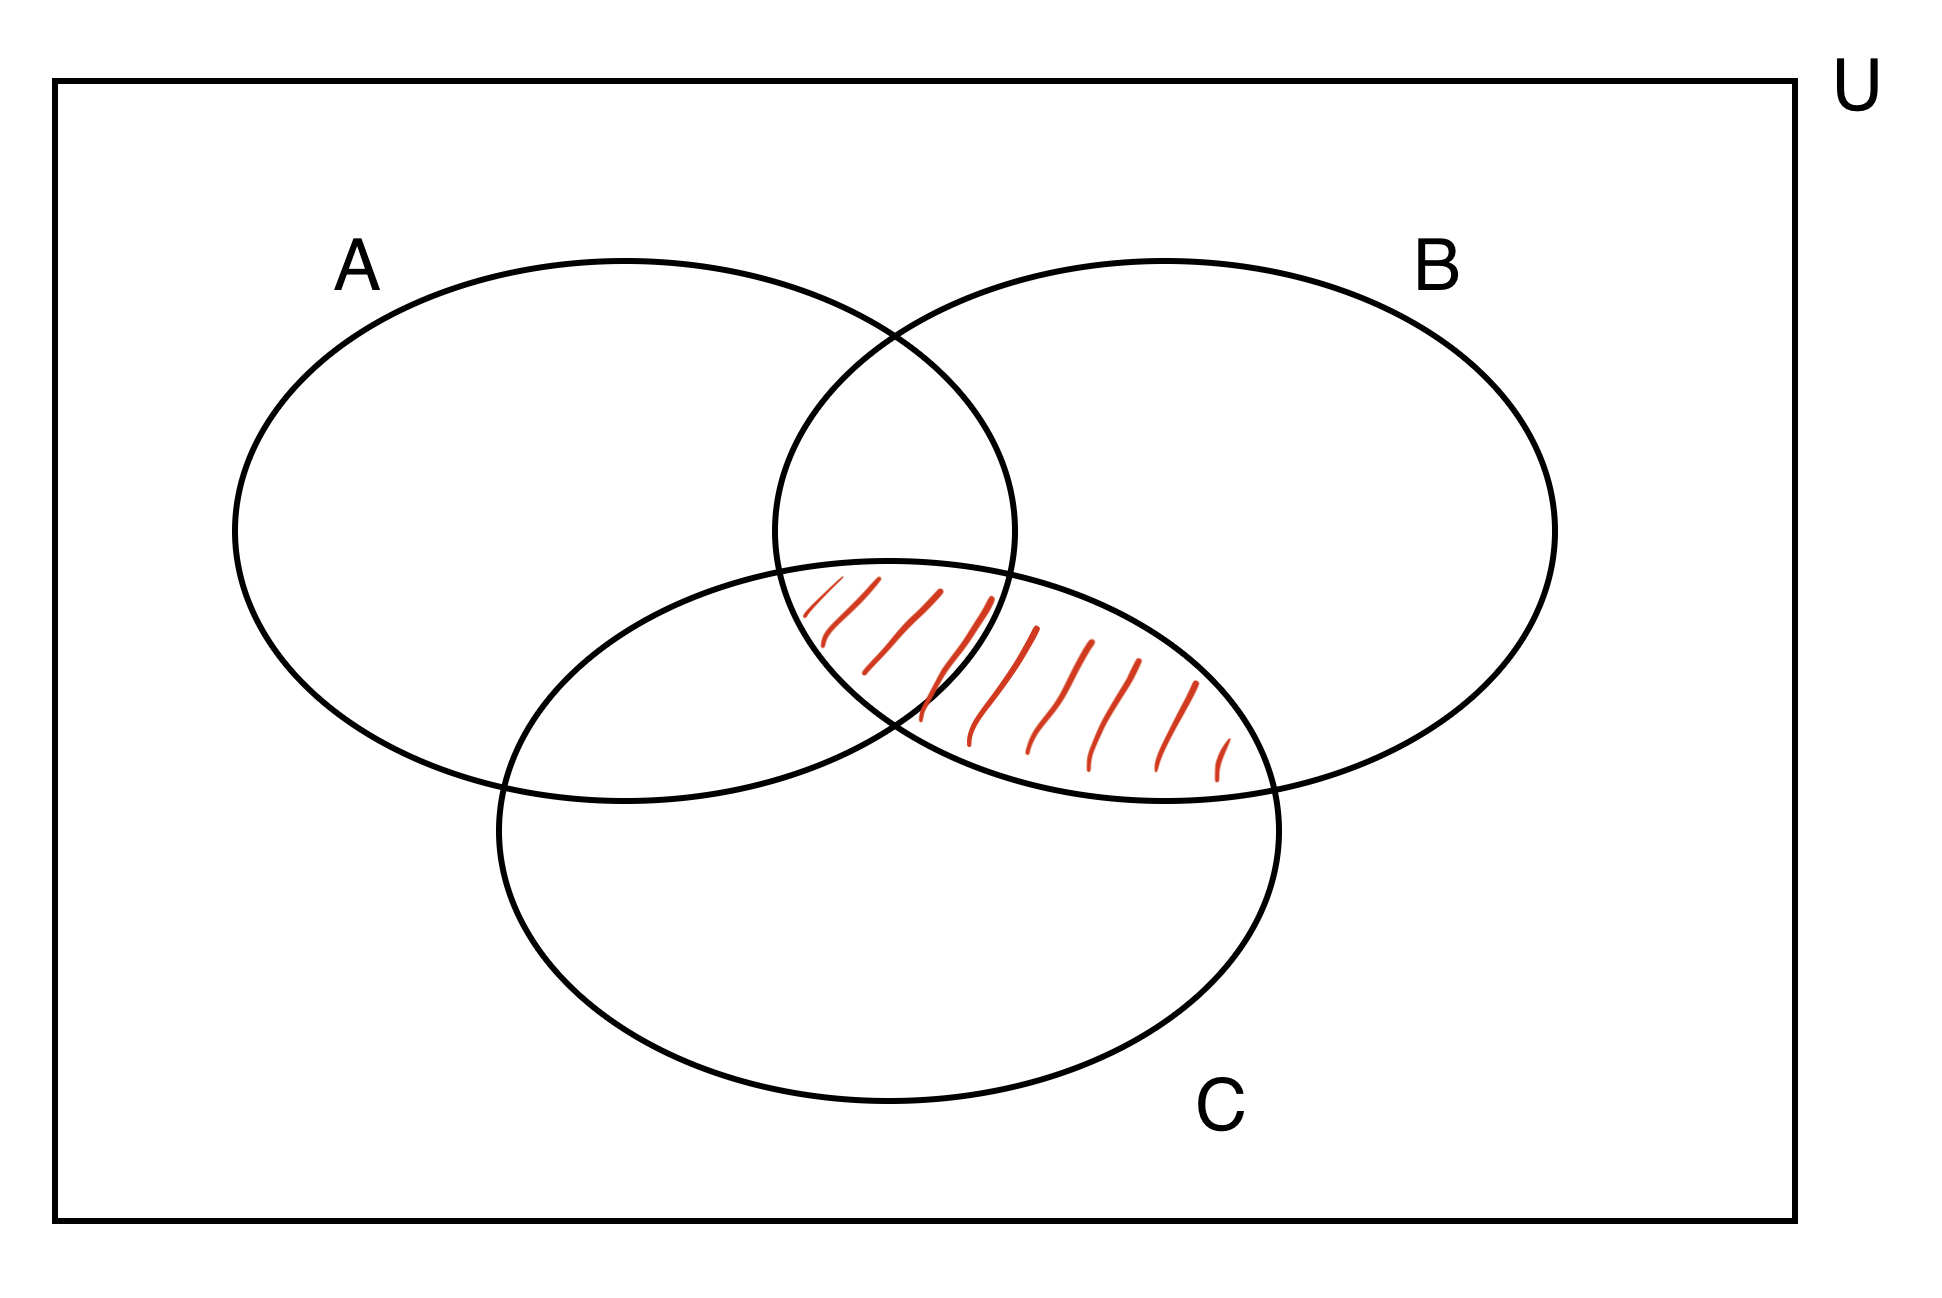
\includegraphics[width=4cm]{Dimostrazione-distibutiva-eulero-venn-2.png}
            \caption{Step 1 - $B \cap C$}
            \label{fig:Dimostrazione-distibutiva-eulero-venn-2}
        \end{subfigure}
        \hfill
        \begin{subfigure}{.3\textwidth}
            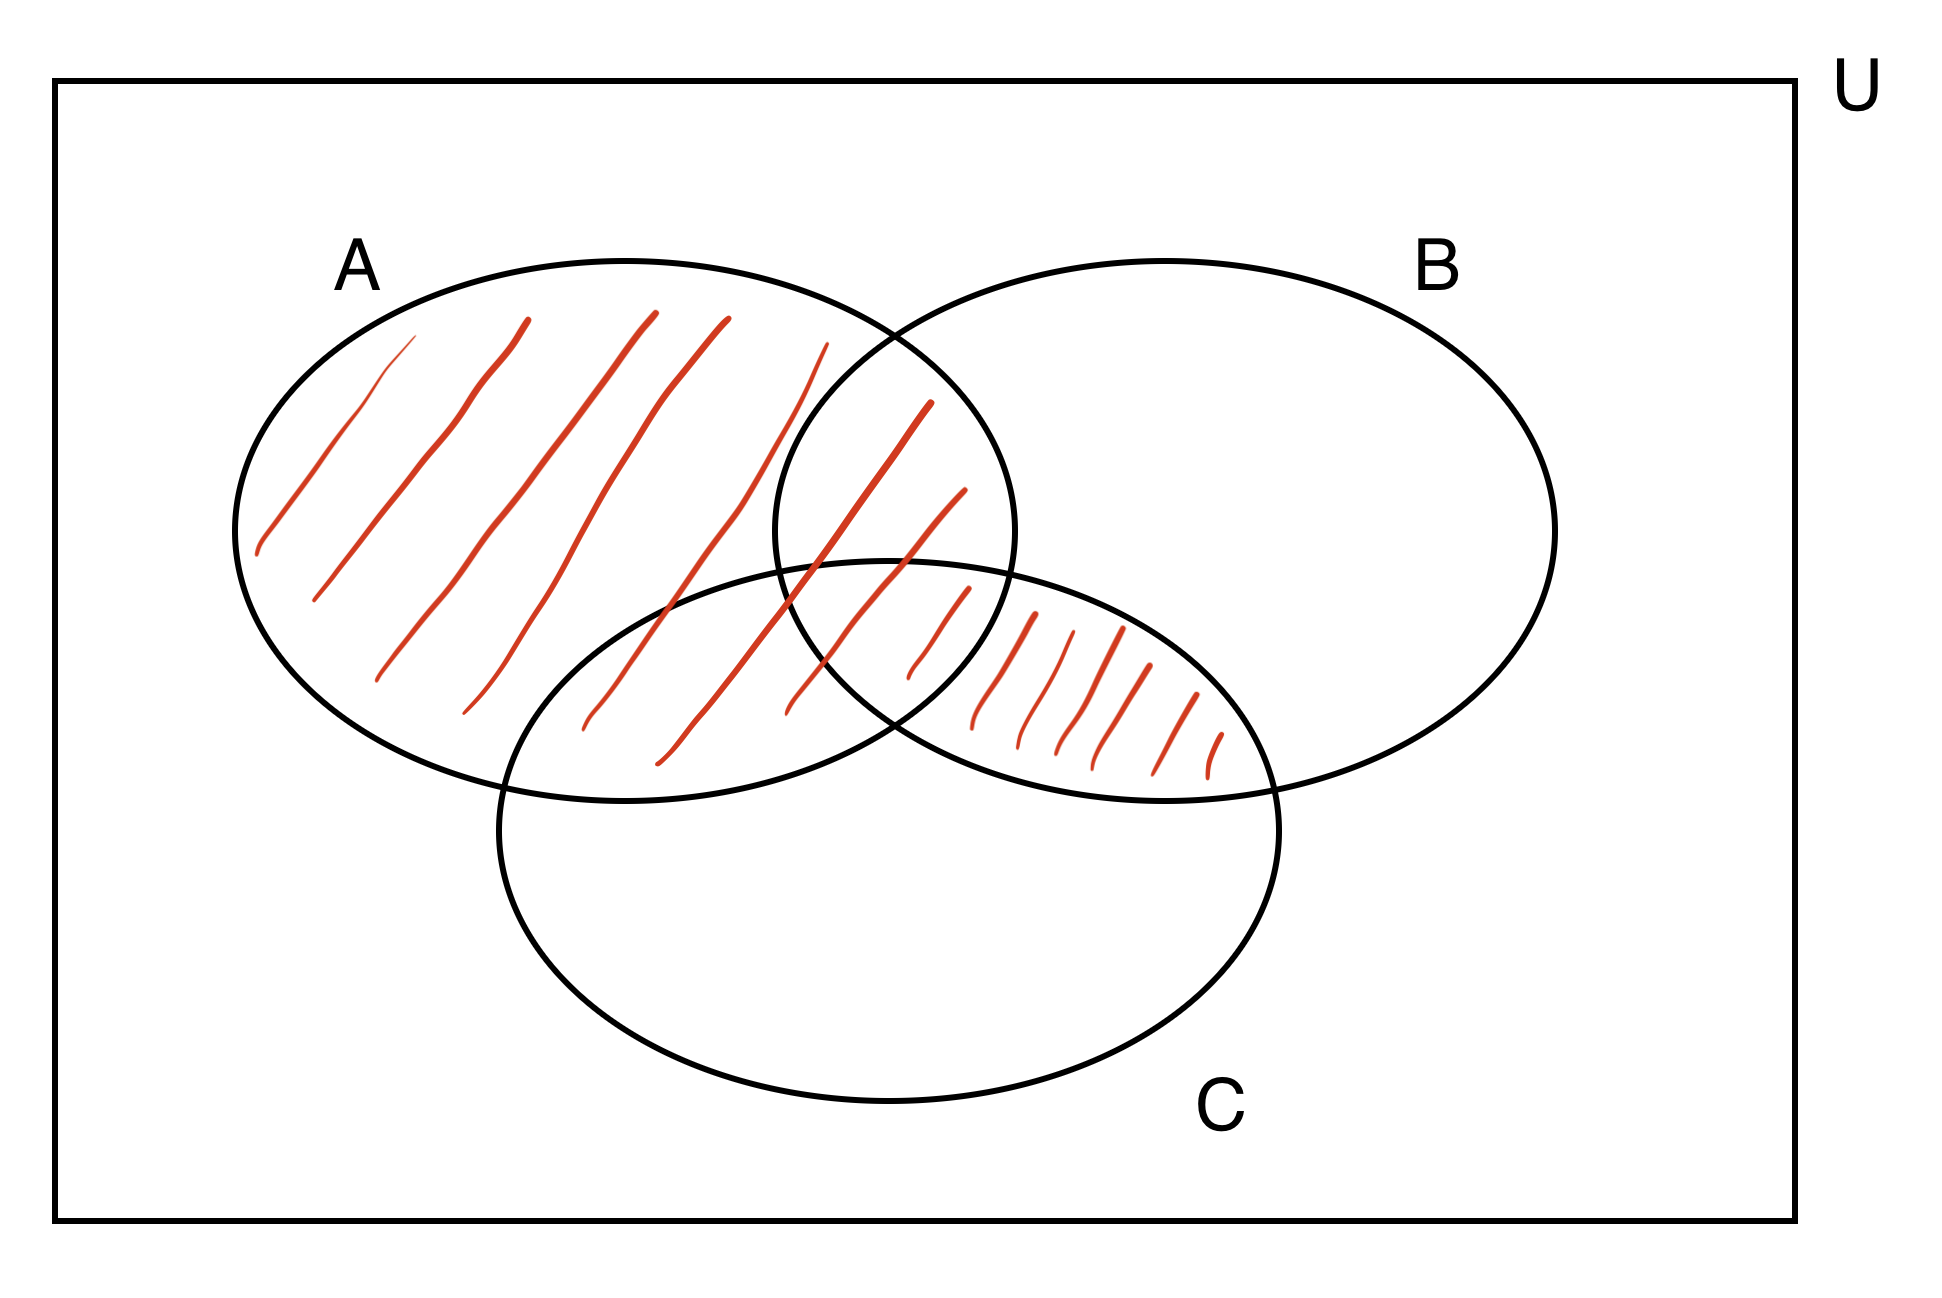
\includegraphics[width=4cm]{Dimostrazione-distibutiva-eulero-venn-3.png}
            \caption{Step 2 - $A \cup (B \cap C)$}
            \label{fig:Dimostrazione-distibutiva-eulero-venn-3}
        \end{subfigure}
    \end{figure}
    \begin{figure}[h!]
        \begin{subfigure}{.3\textwidth}
            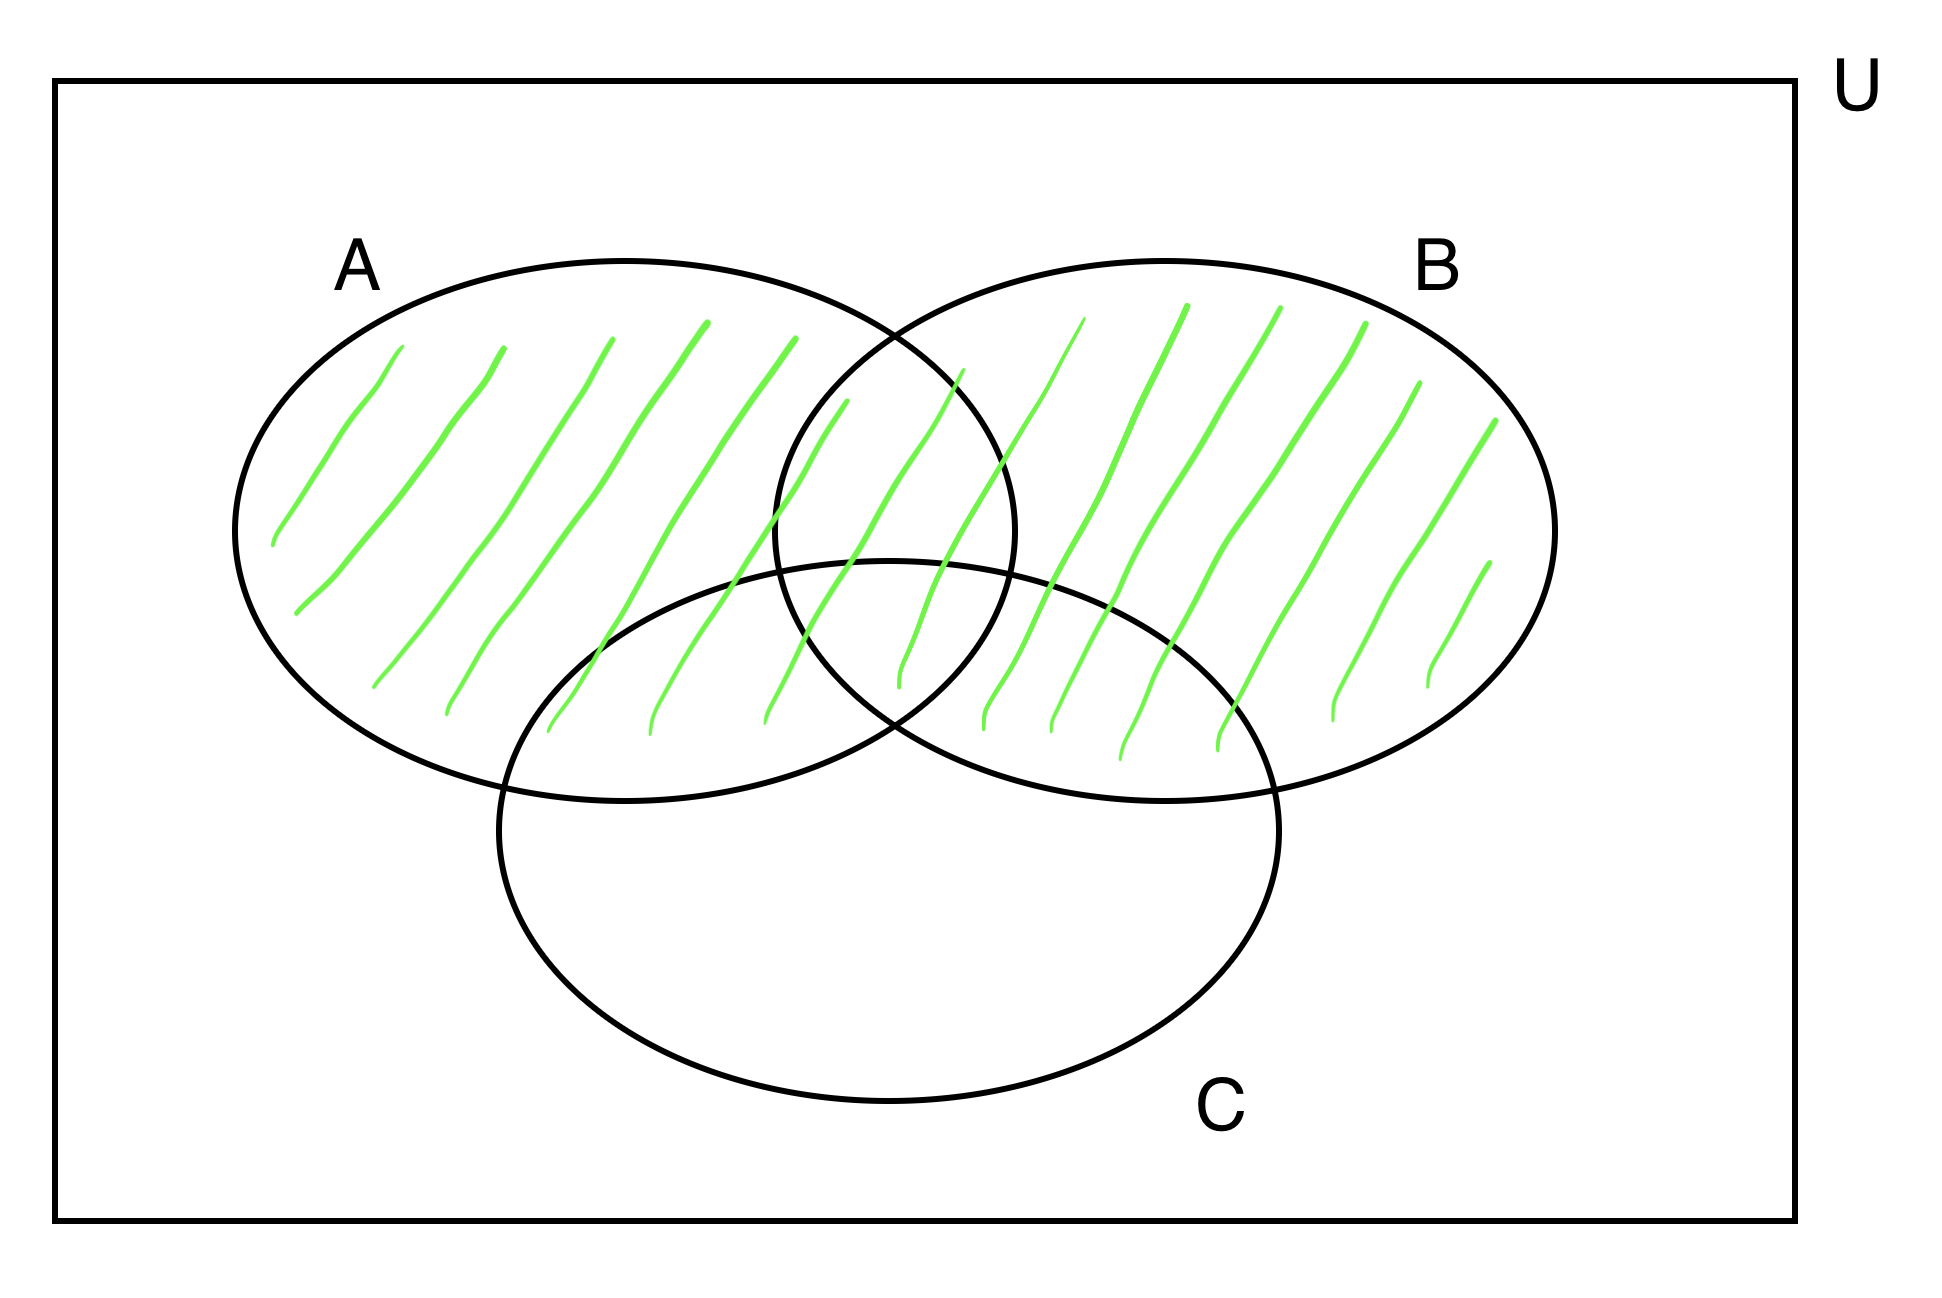
\includegraphics[width=4cm]{Dimostrazione-distibutiva-eulero-venn-4.png}
            \caption{Step 3 - $A \cup B$}
            \label{fig:Dimostrazione-distibutiva-eulero-venn-4}
        \end{subfigure}
        \hfill
        \begin{subfigure}{.3\textwidth}
            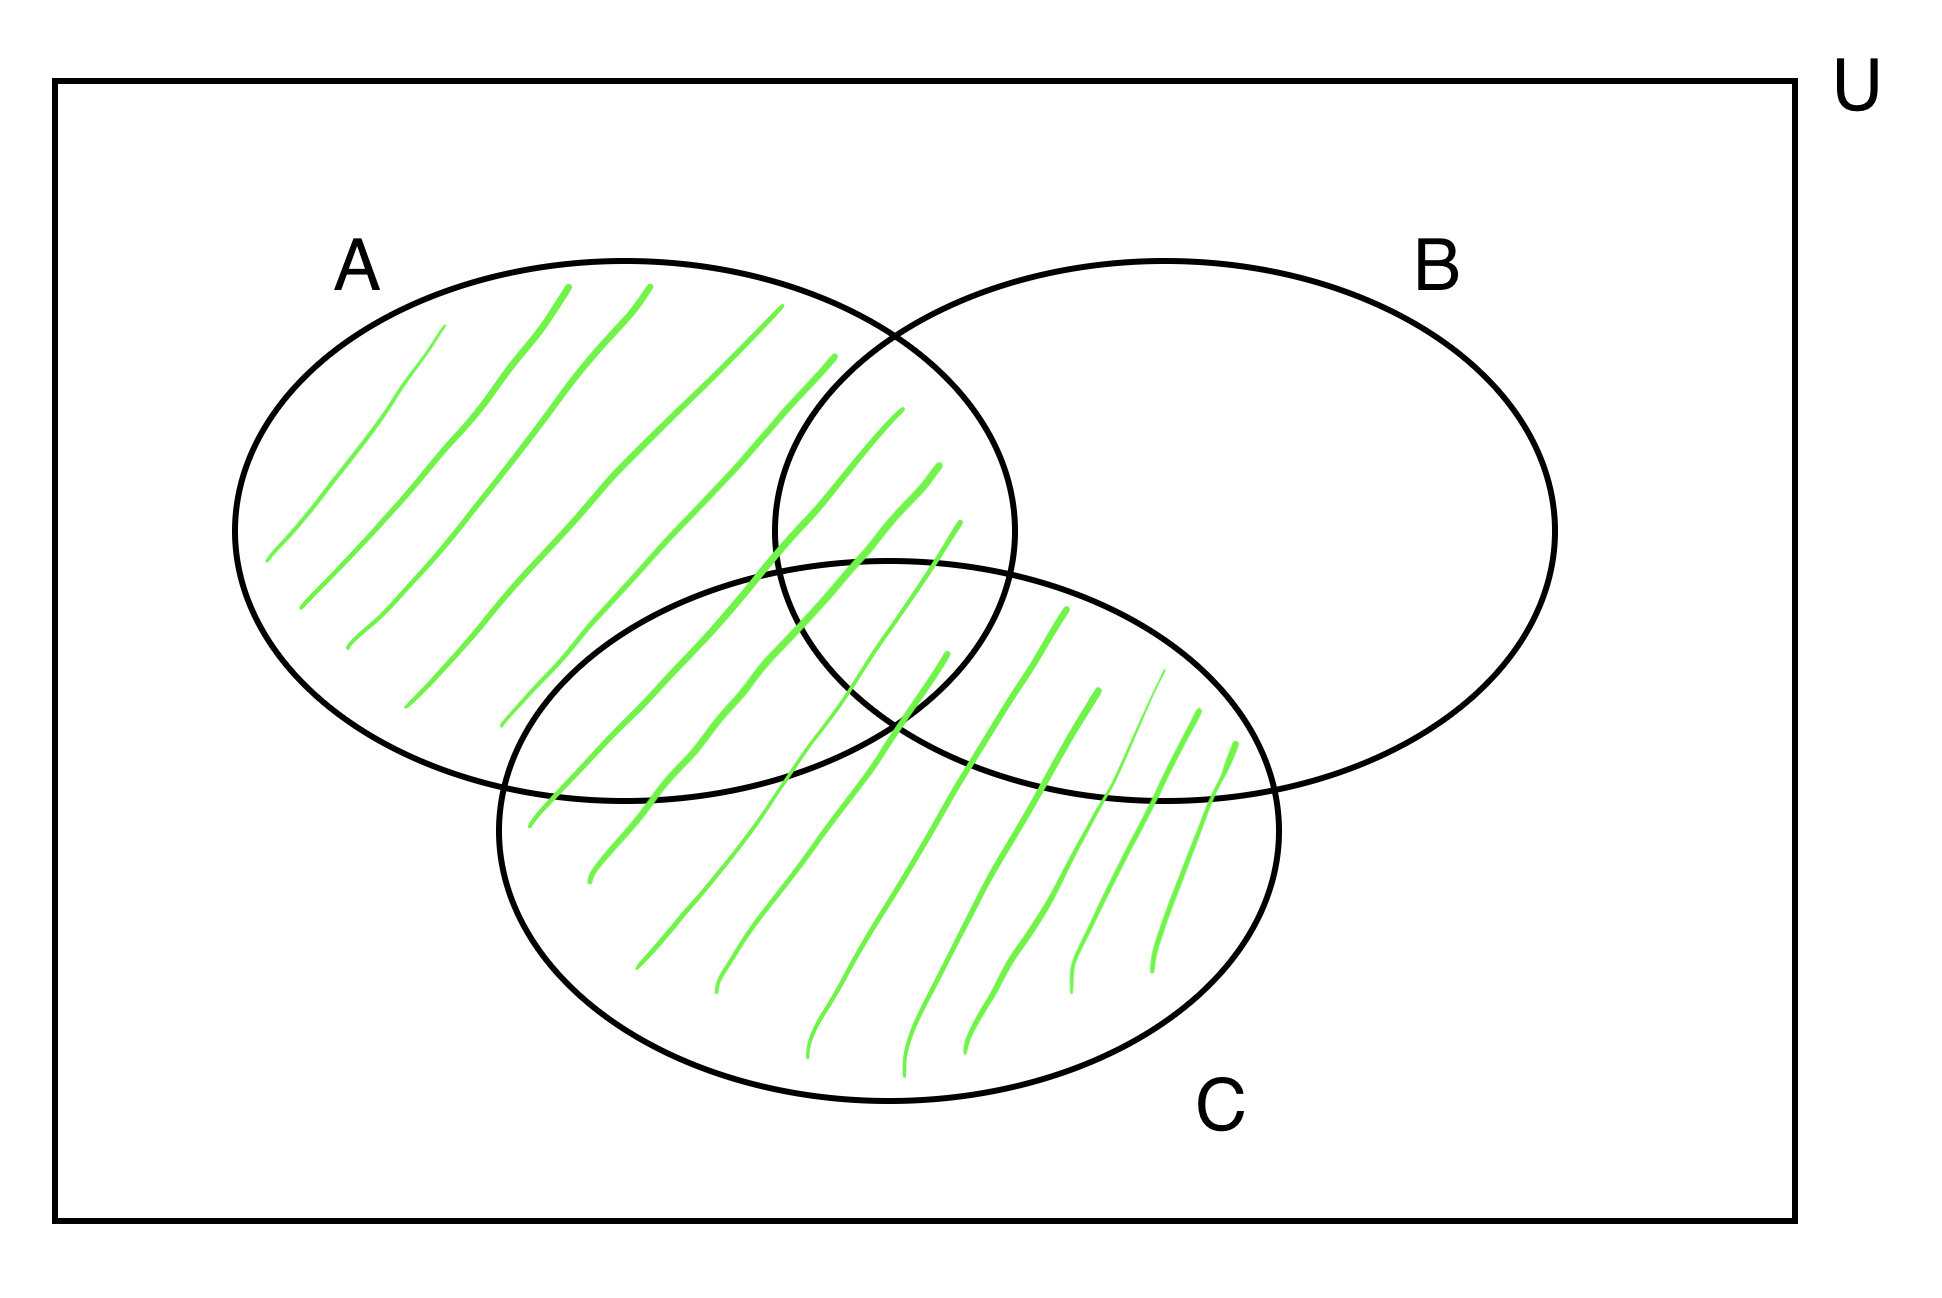
\includegraphics[width=4cm]{Dimostrazione-distibutiva-eulero-venn-5.png}
            \caption{Step 4 - $A \cup C$}
            \label{fig:Dimostrazione-distibutiva-eulero-venn-5}
        \end{subfigure}
        \hfill
        \begin{subfigure}{.3\textwidth}
            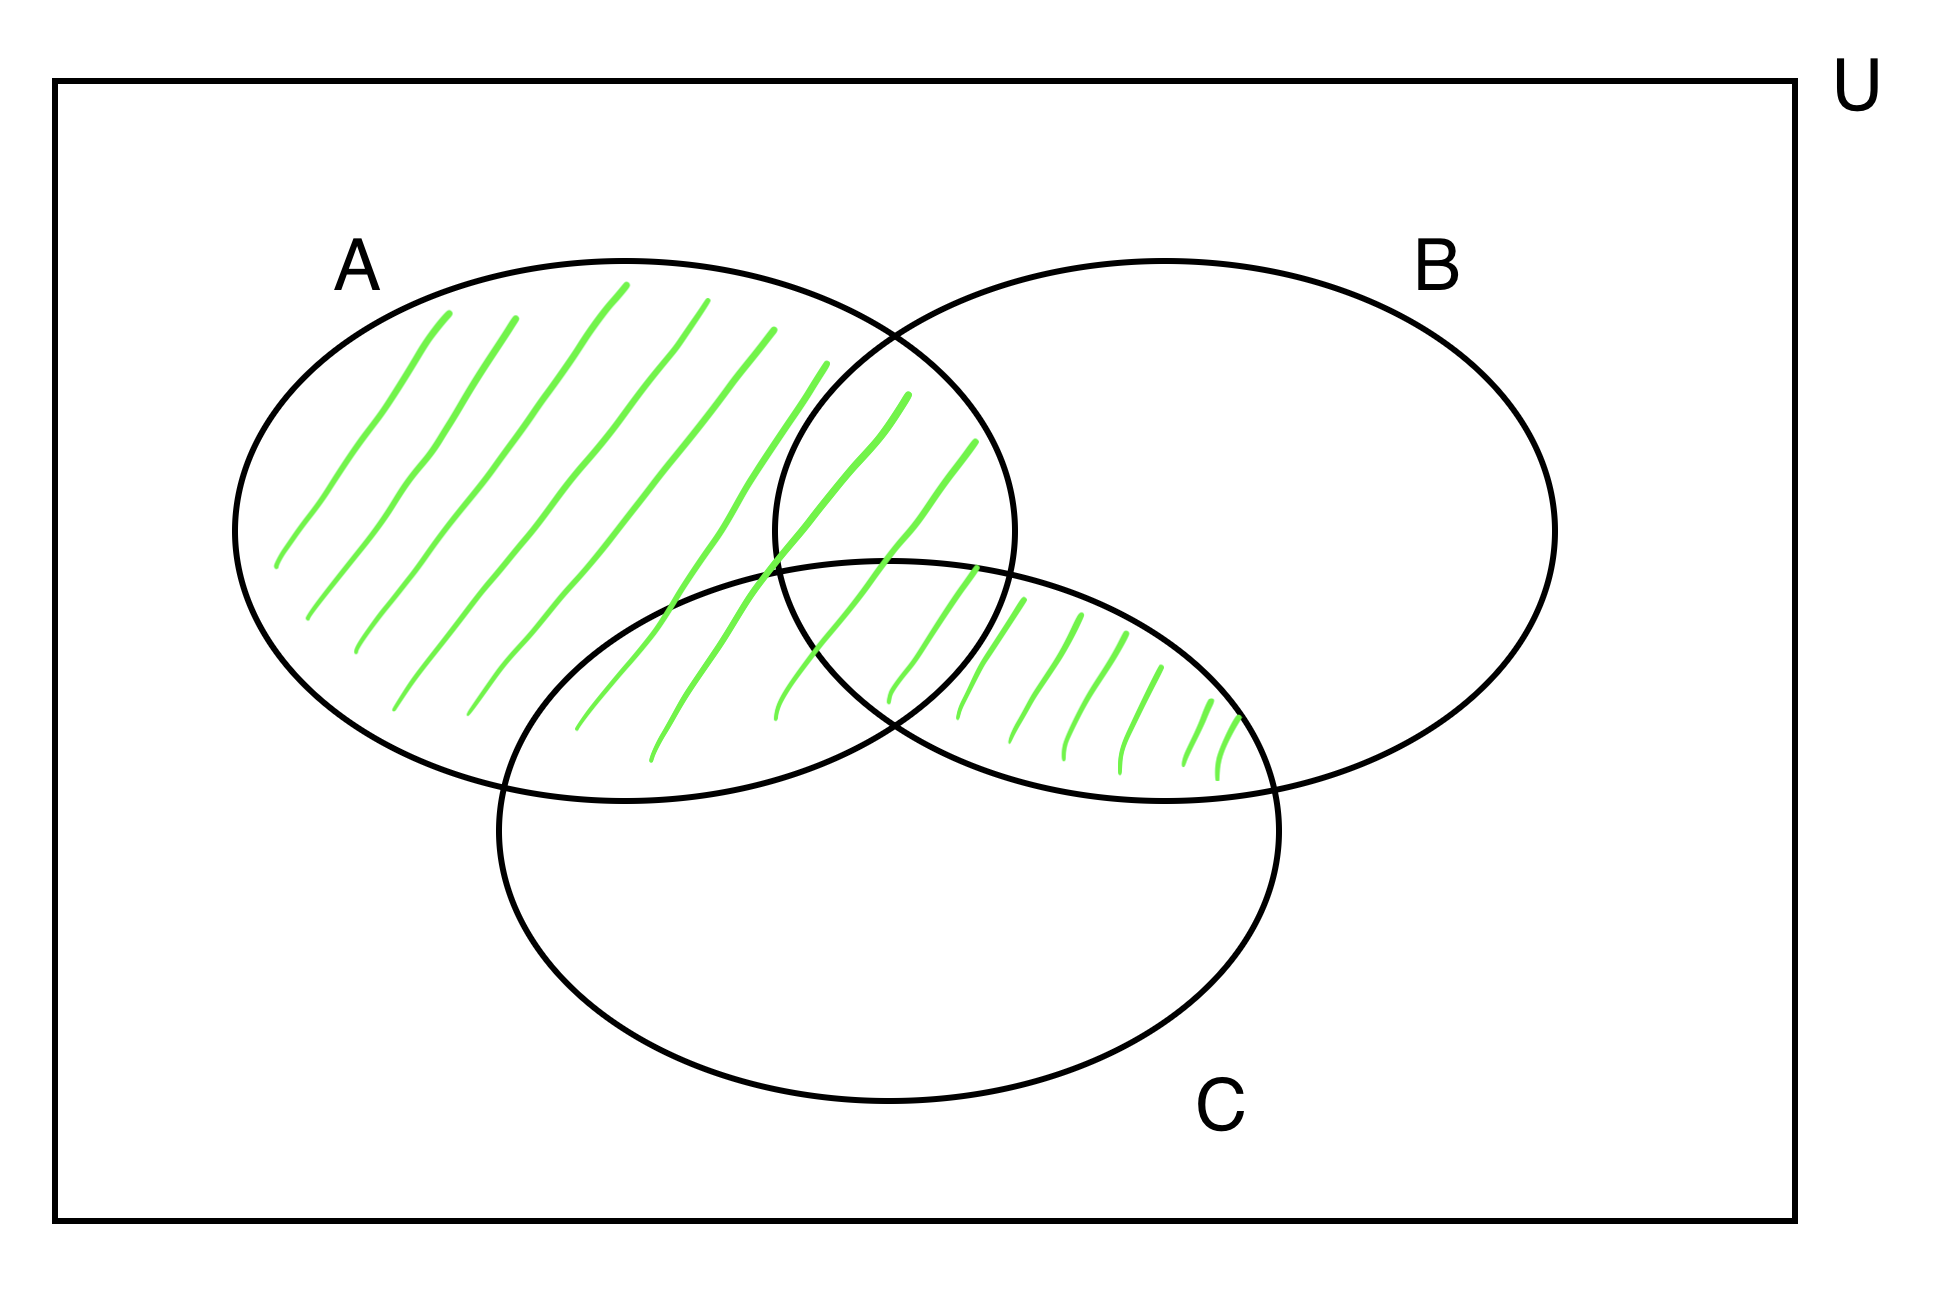
\includegraphics[width=4cm]{Dimostrazione-distibutiva-eulero-venn-6.png}
            \caption{Step 5 - $(A \cup B) \cap (A \cup C)$}
            \label{fig:Dimostrazione-distibutiva-eulero-venn-6}
        \end{subfigure}
    \end{figure}
    \\ Possiamo vedere come lo step 2 (\ref{fig:Dimostrazione-distibutiva-eulero-venn-2}), che rappresenta ciò che dovrebbe essere $A \cup (B \cap C)$ con i diagrammi di eulero-venn, e lo step 5 (\ref{fig:Dimostrazione-distibutiva-eulero-venn-5}), cioè $(A \cup B) \cap (A \cup C)$, siano uguali e quindi possiamo dire che la proprietà e dimostrata.  
\end{example}


\subsubsection{Sostituzione}
Questo tipo di dimostrazione si basa sull'utilizzare leggi preesistenti per dimostrare un'affermazione, scomponendo tale affermazione in modo che si possa ricorrere ad un legge fondamentale.
\begin{example}
    $(A \cup B) \cup C = A \cup (C \cup B)$
    \begin{enumerate}
        \item \textbf{Commutativa}: $(A \cup B) \cup C = A \cup (\mathbf{B \cup C})$
    \end{enumerate}
    L'ipotesi è vera per la proprietà \emph{associativa}.
\end{example}
\begin{example}
    $A \cup (\overline{A} \cap B)$
    \begin{enumerate}
        \item Usando la \textbf{Distributiva} possiamo dividere la prima parte: $(A \cup \overline{A}) \cap (A \cup B) = (A \cup B)$
        \item Usando la proprietà del \textbf{Complemento} $A \cup \overline{A}$ diventa U quindi perché un insieme unito con la sua negazione torna sempre l'universo: $U \cap (A \cup B) = (A \cup B) $
        \item Per la proprietà dell'\textbf{Unità} un insieme A unito con l'universo U è uguale a l'insieme stesso quindi: $A \cup B = A \cup B$
    \end{enumerate}
    L'ipotesi è così verificata.
\end{example}
 
\subsubsection{Discorsiva}
Esempio di dimostrazione della proprietà distributiva:
\begin{equation}
	A \cup (B \cap C) = (A \cup B) \cap (A \cup C)
\end{equation}
Teniamo conto che: $X = Y \iff (X \subseteq Y) \land (Y \subseteq X)$.\\
Andiamo a questo punto a sostituire X con la prima parte della proprietà distributiva, $A \cup (B \cap C)$ e Y con la seconda $(A \cup B) \cap (A \cup C)$. 
Applicando la considerazione scritta sopra otteniamo due condizione che devono entrambi essere vere per far si che la condizione di uguaglianza iniziale $A \cup (B \cap C) = (A \cup B) \cap (A \cup C)$ sia vera e quindi la proprietà sia verificata. Queste due condizioni sono:
\begin{itemize}
    \item $A \cup (B \cap C) \subseteq (A \cup B) \cap (A \cup C)$ - \underline{Dimostrazione 1°}
    \item $(A \cup B) \cap (A \cup C) \subseteq A \cup (B \cap C)$ - \underline{Dimostrazione 2°}
\end{itemize}
\textbf{Dimostrazione 1°}: $A \cup (B \cap C) \subseteq (A \cup B) \cap (A \cup C)$\\
\textit{Ricordiamo che un insieme $W \subseteq Z$ per ogni $x \in W$ e $z \in Z$.}\\
Sostituendo la W con la prima parte, $A \cup (B \cap C)$, e la Z con la seconda, $(A \cup B) \cap (A \cup C)$ possiamo scrivere che $y \in A \cup (B \cap C)$. Per la definizione di unione possiamo distinguere in 2 casi.
\begin{center}
    (1a) $y \in A$ \hspace{.5cm}  (1b) $y \in (B \cap C)$ \\
\end{center}
Da qui il nostro obbiettivo è far valere per entrambi i casi che $y \in (A \cup B) \cap (A \cup C)$.
\begin{itemize}
    \item \textbf{Caso 1a:} $y \in A$
    \begin{enumerate}
        \item Per questo caso possiamo vedere come, per la definizione di unione, aggiungendo qualsiasi cosa all'insieme A l'appartenenza di y rimarrà invariata. Quindi $y \in A \cup B$, $y \in A \cup C$.
        \item Da qui per la definizione di intersezione\footnote{\textit{($y \in W \cap Z, \iff y \in W \: e \: y \in Z$)}} $y \in (A \cup B) \cap (A \cup C)$. Caso dimostrato. $\blacksquare$
    \end{enumerate}
    \item \textbf{Caso 1b:} $y \in (B \cap C)$
    \begin{enumerate}
        \item Siccome $x \in B \cap C$, per definizione di intersezione si ha che $x \in B$ e che $x \in C$.
        \item Dato che $x \in B$, a sua volta ha che $x \in A \cup B$.
        \item Analogamente, dato che $x \in C$, per definizione di unione si ha che $x \in A \cup C$.
        \item Ma allora, visto che x appartiene a entrambi questi insiemi deve appartenere anche alla
        loro intersezione, ovvero $y \in (A \cup B) \cap (A \cup C)$. Caso dimostrato. $\blacksquare$
    \end{enumerate}
\end{itemize}
\textbf{Dimostrazione 2°}: $(A \cup B) \cap (A \cup C) \subseteq A \cup (B \cap C)$ \\
Come per la dimostrazione 1° andiamo a prendere qualsiasi elemento $y \in (A \cup B) \cap (A \cup C)$.\\
Da qui per la definizione di intersezione $y \in (A \cup B)$ e $y \in (A \cup B)$ che ci permette di conseguenza di distinguere 4 casi:
\begin{center}
    (1) $y \in A$ e $y \in A$ \hfill
    (2) $y \in A$ e $y \in B$ \hfill
    (3) $y \in C$ e $y \in A$ \hfill
    (4) $y \in B$ e $y \in C$
\end{center}
Però possiamo racchiudere le prime 3 con $y \in A$ e l'ultima come $y \notin A$. Quindi abbiamo due possibilità disgiunti fra loro.
\begin{center}
    (2a) $y \in A$ \hspace{.5cm}  (2b) $y \notin A$ \\
\end{center}
In entrambi i casi bisogna arrivare a dimostrare che $y \in A \cup (B \cap C)$.
\begin{itemize}
    \item \textbf{Caso 2a:} $y \in A$
    \begin{enumerate}
        \item Essendo che $y \in A$ allora per definizione di unione $y \in A \cup (B \cap C)$. Caso dimostrato. $\blacksquare$
    \end{enumerate}
    \item \textbf{Caso 2b:} $y \notin A$
    \begin{enumerate}
        \item Dato che $y \in A \cup B$ ma $y \notin A$, allora necessariamente $y \in B$.
        \item Analogamente, data che $y \in A \cup C$ ma $y \notin A$, allora $y \in C$.
        \item Visto che y apparitene sia a B che a C deve per forza appartenere alla loro intersezione, quindi $y \in (B \cap C)$.
        \item A questo punto per definizione di unione $y \in A \cup (B \cap C)$. Caso dimostrato. $\blacksquare$
    \end{enumerate}
\end{itemize}
Non avendo nessun' altro caso da dimostrare abbiamo concluso la dimostrazione. $\blacksquare$

\subsection{Prodotto Cartesiano}
Prendendo 2 insiemi A, B il loro prodotto cartesiano si definisce come:
\begin{center}
    $A \: X \: B = \{(a, b) \: | \: a \in A, \: b \in B\}$
\end{center}
\begin{example}
    Esempio prodotto cartesiano:\\\\
    $A = \{501234, 501227, 678980\}$ N. matricola \hspace{1cm}
    $B = \{18, 19, 20, ..., 30L\}$ Voti \\
    $A \: X \: B = \{(501234, 18), (501234, 19), ..., (678980, 30L)\}$\\ \\
    I sotto insiemi che si vanno a creare con il prodotto cartesiano si indicano con le parentesi tonde "(...)" e possono essere di due tipi:
    \begin{itemize}
        \item \textbf{Coppia Ordinata:} si tiene conto dell'ordinamento degli elementi. Ess: $(a, b) \neq (b, a)$.
        \item \textbf{Coppia Non Ordinata:} non si tiene conto dell'ordinamento degli elementi. Ess: $(a, b) = (b, a)$.
\end{itemize}
\end{example}

\subsection{Insiemi di insiemi}
\begin{definition}[Insieme]
Un insieme di insieme è quando uno o più elementi di un insieme è a sua volta un insieme.
\end{definition}
\begin{example}
Esempi insiemi di insiemi:
    \begin{itemize}
        \item $X = \{a, \{a, b, c\}, \{a, \{b\}\}, \{\{c\},d\}\}$
        \item $N = \{\{\}, \{\{\}\}, \{\{\{\}\}\}, \{\{\{\{\}\}\}\}, ...\} = \mathbb{N}$
    \end{itemize}
\end{example}

\begin{definition}[Insieme delle parti]
L'insieme della parti, per esempio di A, si indica come P(A) e si definisce come tutti i possibili sottoinsiemi di A. $P(A) = \{x \subseteq A\}$. La \textbf{cardinalità} nell'insieme delle parti si calcola come: $P(A) = 2^{|A|}$
\end{definition}
\begin{example}
    Con $A = \{a, b, c\}$, $\wp(A) = \{\O, \{a\}, \{b\}, \{c\}, \{a, b\}, \{a, c\}, \{c, b\}, \{a, b, c\}\}$
\end{example}
